\documentclass{article}
\usepackage[utf8]{inputenc}
\usepackage[margin=0.5in]{geometry}
\usepackage{graphicx}
\usepackage{amsmath}
\usepackage{ dsfont }

\graphicspath{ {../figs/} }


\title{Problem Set 1: Quantitative Economics (ECON 8185-001)}
\author{Teerat Wongrattanapiboon}
\date{15 December 2021}

\begin{document}

	\maketitle
	
	\noindent\textbf{\Large Stochastic Growth Model} \\
	
	We want to compute the equilibria of the following growth model:
	
	$$\max_{c_{t},x_{t},l_{t}} E\sum_{t=0}^{\infty}\beta^{t}[\log(c_{t}) + \psi \log(l_{t})]N_{t}$$
	
	$$\text{s.t. } c_{t} + x_{t} = k_{t}^\theta\Big( (1+\gamma_{z})^{t}z_{t}h_{t} \Big)^{1-\theta}$$
	$$N_{t+1}k_{t+1} = [(1-\delta)k_{t} + x_{t}]N_{t}$$
	$$\log(z_{t}) = \rho \log(z_{t-1})+\epsilon_{t}, \epsilon \sim N(0,\sigma^{2})$$
	$$h_{t}+l_{t} = 1$$
	$$c_{t},x_{t} \geq 0,$$
	
	where $N_{t} = (1+\gamma_{n})^{t}$. First, we detrend the technological progress. The resource constraint can be written as
	
	$$c_{t}+x_{t} = (1+\gamma_{z})^{t}\Big( \frac{k_{t}}{(1+\gamma_{z})^{t}} \Big)^{\theta}(z_{t}h_{t})^{1-\theta}.$$
	
	Then, define $\hat{c_{t}} = \frac{c_{t}}{(1+\gamma_{z})^{t}}$, $\hat{x_{t}} = \frac{x_{t}}{(1+\gamma_{z})^{t}}$, $\hat{k_{t}} = \frac{k_{t}}{(1+\gamma_{z})^{t}}$, and $\hat{\beta} = \beta(1+\gamma_{n})$ and rewrite our original model to be
	
	$$\max_{\hat{c_{t}},\hat{k_{t+1}},h_{t}} E\sum_{t=0}^{\infty}\hat{\beta}^{t}[\log((1+\gamma_{z})^{t}\hat{c_{t}}) + \psi \log(1-h_{t})]$$
	
	$$\text{s.t. } \hat{c_{t}} + \hat{x_{t}} = k_{t}^\theta(e^{z_{t}}h_{t})^{1-\theta}$$
	$$(1+\gamma_{n})(1+\gamma_{z})\hat{k}_{t+1} = (1-\delta)\hat{k_{t}} + \hat{x_{t}}$$
	$$z_{t} = \rho z_{t-1}+\epsilon_{t}, \epsilon \sim N(0,\sigma^{2})$$
	$$c_{t},x_{t} \geq 0.$$
	
	By substituting in $c_{t}$ and $x_{t}$, we obtain the following Bellman's equation:
	
	$$V(\hat{k}_{t},z_{t}) = \max_{\hat{k}_{t+1},h_{t}}\Big\{ \log \Big( (\hat{k}_{t})^{\theta} (e^{z_{t}}h_{t})^{1-\theta} - (1+\gamma_{n})(1+\gamma_{z})\hat{k}_{t+1} + (1-\delta)\hat{k}_{t} \Big) \Big\} + \psi\log(1-h_{t}) + \hat{\beta}\mathds{E}\big[ V(\hat{k}_{t+1},z_{t+1}) \big].$$
	
	Given this Bellman's equation, we can write the FOCs and envelope condition as:
	
	$$\boldsymbol{[\hat{k}_{t+1}]:} \frac{-(1+\gamma_n)(1+\gamma_z)}{(\hat{k}_{t})^{\theta} (e^{z_{t}}h_{t})^{1-\theta} - (1+\gamma_{n})(1+\gamma_{z})\hat{k}_{t+1} + (1-\delta)\hat{k}_{t}} + \hat{\beta}\mathds{E}\Big[ \frac{\partial V(\hat{k}_{t+1},z_{t+1})} {\partial \hat{k}_{t+1}} \Big] = 0$$
	
	$$\boldsymbol{[h_t]:} \frac{(1-\theta)\hat{k}_{t}^{\theta}e^{z_{t}(1-\theta)}h_{t}^{-\theta}}{(\hat{k}_{t})^{\theta} (e^{z_{t}}h_{t})^{1-\theta} - (1+\gamma_{n})(1+\gamma_{z})\hat{k}_{t+1} + (1-\delta)\hat{k}_{t}} - \frac{\psi}{(1-h_{t})} = 0$$
	
	$$\boldsymbol{[ENV]:} \frac{\partial V(\hat{k}_{t+1},z_{t+1})} {\partial \hat{k}_{t+1}} = \frac{\theta\hat{k}_{t+1}^{\theta-1}(e^{z_{t+1}}h_{t+1})^{1-\theta}+1-\delta}{(\hat{k}_{t+1})^{\theta} (e^{z_{t+1}}h_{t+1})^{1-\theta} - (1+\gamma_{n})(1+\gamma_{z})\hat{k}_{t+2} + (1-\delta)\hat{k}_{t+1}}.$$
	
	Combining the FOC for $\hat{k}_{t+1}$ and the envelope condition, we have the following Euler equation:
	
	$$\frac{(1+\gamma_n)(1+\gamma_z)}{(\hat{k}_{t})^{\theta} (e^{z_{t}}h_{t})^{1-\theta} - (1+\gamma_{n})(1+\gamma_{z})\hat{k}_{t+1} + (1-\delta)\hat{k}_{t}} = \hat{\beta}\mathds{E}\Big[ \frac{\theta\hat{k}_{t+1}^{\theta-1}(e^{z_{t+1}}h_{t+1})^{1-\theta}+1-\delta}{(\hat{k}_{t+1})^{\theta} (e^{z_{t+1}}h_{t+1})^{1-\theta} - (1+\gamma_{n})(1+\gamma_{z})\hat{k}_{t+2} + (1-\delta)\hat{k}_{t+1}} \Big].$$
	
	Also, notice that the FOC for $h_{t}$ governs the labor-consumption choices. Therefore, we can solve for capital and labor in steady state with the following two equations:
	
	$$\hat{\beta}(\theta\hat{k}_{ss}^{\theta-1}(e^{0}h_{ss})^{1-\theta}+1-\delta) - (1+\gamma_n)(1+\gamma_z) = 0$$
	
	$$\frac{(1-\theta)\hat{k}_{ss}^{\theta}e^{0}h_{ss}^{-\theta}}{(\hat{k}_{ss})^{\theta} (e^{0}h_{ss})^{1-\theta} - (1+\gamma_{n})(1+\gamma_{z})\hat{k}_{ss} + (1-\delta)\hat{k}_{ss}} - \frac{\psi}{(1-h_{ss})} = 0$$
	
	With the following calibration, we can compute the steady state of this economy:
	
	\begin{center}
		\begin{tabular}{| c | c |  }
		\hline
 		Parameter & Value \\
 		\hline 
 		$\theta$ & 0.35  \\  
 		$\delta$ & 0.0464 \\
 		$\gamma_z$ & 0.016 \\
 		$\gamma_n$ & 0.015 \\
 		$\delta$ & 0.0464 \\
 		$\beta$ & 0.9722 \\
 		$\psi$ & 2.24 \\
 		$\rho$ & 0.2 \\
 		$\sigma$ & 0.5 \\
 		\hline    
		\end{tabular}
	\end{center}
	
	\begin{center}
		\begin{tabular}{| c | c |  }
		\hline
 		Variable & Steady-State Value \\
 		\hline 
 		$k_{ss}$ & 2.304 \\  
 		$h_{ss}$ & 0.292 \\
 		$l_{ss}$ & 0.708 \\
 		$c_{ss}$ & 0.423 \\
 		\hline    
		\end{tabular}
	\end{center}
	
	\noindent\textbf{\Large Value Function Iteration} \\
	
	For the Value Function Iteration, I constructed $1000$ grids of capital around steady states level of capital, with the range $[0.5*k_{ss}, 1.5*k_{ss}]$, and $5$ grids for production shocks, which are discretized using Tauchen's method. \\
	
	 I first solved the static problem from Intratemporal equation with Newton Root method to find optimal level of labor choice over the multidimensional grid ($k \times z \times k'$) to speed up the algorithm. The optimal policy functions for capital, consumption, and labor are plotted below: \\
	 
	 \noindent\textbf{\Large Linear Quadratic Approximation} \\
	 
	 Here, I assumed that my return function depends on hours ($h_{t}$), capital today ($k_{t}$), and capital tomorrow ($k_{t+1}$). \\
	 
	 \textbf{Step 1:} Compute the steady state level of variables with Nonlinear solver. This step is done in the same manner as in VFI. \\
	 
	 \textbf{Step 2:} Express the return function with Linear-Quadratic \\
	 
	 $$ r \left( X_{t} = \begin{bmatrix} \hat{k}_{t} \\ \hat{z}_{t} \\ 1  \end{bmatrix}, u_{t} = \begin{bmatrix} \hat{k}_{t+1} \\ h_{t}  \end{bmatrix} \right) = \log\Big( (e^{\hat{z}_{t}}\hat{k}_{t})^\theta(h_{t})^{1-\theta} - (1+\gamma_{n})(1+\gamma_{z})\hat{k}_{t+1} + (1-\delta)\hat{k}_{t} \Big) + \psi \log(1-h_{t})$$
	 
	 $$\text{s.t. } \begin{bmatrix} \hat{k}_{t+1} \\ \hat{z}_{t+1} \\ 1  \end{bmatrix} = \begin{bmatrix} 0 & 0 & 0 \\ 0 & \rho & 0 \\ 0 & 0 & 1  \end{bmatrix}\begin{bmatrix} \hat{k}_{t} \\ \hat{z}_{t} \\ 1  \end{bmatrix} + \begin{bmatrix} 1 & 0 \\ 0 & 0 \\ 0 & 0  \end{bmatrix}\begin{bmatrix} \hat{k}_{t+1} \\ h_{t}  \end{bmatrix} + \begin{bmatrix} 0 \\ 1 \\ 0 \end{bmatrix}\epsilon_{t+1}.$$
	 
	 Next, I applied Kydland and Prescott's method to obtain matrices $R$, $Q$, and $W$ by implementing second order linearization around steady state. So now we can express the above problem in the following set-up:
	 
	 $$\max_{ \{u_{t} \}_{t=0}^{\infty}} \mathds{E}_{0}\left[ \sum_{t=0}^{\infty}\hat{\beta}^{t} \{ X_{t}'QX + u_{t}'Ru_{t} + 2X_{t}'Wu_{t} | X_{0} \} \right]$$
	 
	 $$\text{s.t. } X_{t+1} = AX_{t} + Bu_{t} + C\epsilon_{t},$$
	 
	 $$X_{0} \text{ is given. }$$
	 
	 Then we map this problem into undiscounted problem using below transformations:
	 
	 $$\tilde{X}_{t} = \beta^{\frac{t}{2}}X_{t}$$
	 
	 $$\tilde{u}_{t} = \beta^{\frac{t}{2}}(u_{t} + R^{-1}W'X_{t})$$
	 
	 $$\tilde{A} = \sqrt{\beta}(A - BR^{-1}W')$$
	 
	 $$\tilde{B} = \sqrt{\beta}B$$
	 
	 $$\tilde{Q} = Q - WR^{-1}W'.$$
	 
	 \textbf{Step 3:} Obtain a policy function by using convergence of Riccati equation \\
	 
	 Given the initial $P_{0}$ and $F_{0}$, \\
	 
	 1) Update $P_{n}$ and $F_{n}$ with the following update rules
	 
	 $$P_{n+1} = \tilde{Q} + \tilde{A}'P_{n}\tilde{A} = \tilde{A}'P_{n}\tilde{B}(R + \tilde{B}'P_{n}\tilde{B})^{-1}\tilde{B}'P_{n}\tilde{A}$$
	 $$F_{n+1} = (R + \tilde{B}'P_{n}\tilde{B})^{-1}\tilde{B}'P_{n}\tilde{A}.$$
	 
	 2) Iterate until both equations satisfy their convergence criteria at the same time. \\
	 
	 3) Set $F = F_{n} + R^{-1}W'$ and $P = P_{n}$. \\
	 
	 4) Lastly, our optimal policy function is 
	 
	 $$u_{t} = -F\begin{bmatrix} \hat{k}_{t} \\ \hat{z}_{t} \\ 1  \end{bmatrix}$$
	 
	 Below I plotted the optimal capital and labor policy functions, with three different labor productivity shocks (high, low, steady-state). \\
	 
	 \begin{figure}[htbp]
		\centering
		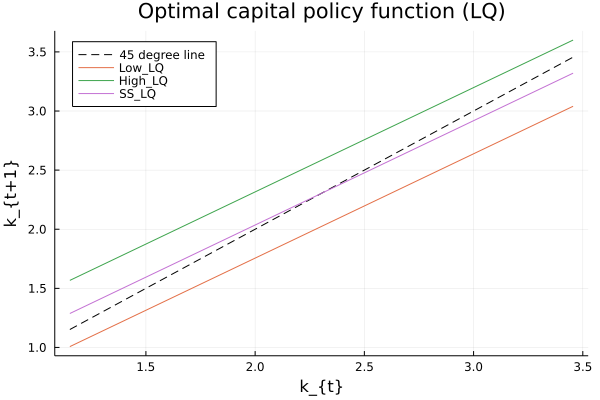
\includegraphics[scale=0.5]{kpol_LQ.png}
		\caption{Optimal policy function for capital from LQ method}
	\end{figure}
	
	\begin{figure}[htbp]
		\centering
		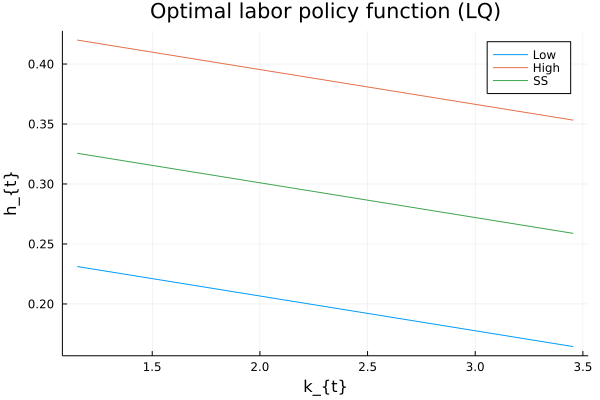
\includegraphics[scale=0.5]{hpol_LQ.png}
		\caption{Optimal policy function for labor from LQ method}
	\end{figure}
	 
	 
	 
	 \noindent\textbf{\Large Vaughan's Method} \\
	 
	 Next we will implement Vaughan's method. All the steps are the same as in LQ method up to obtaining the undiscounted problem. Then we define the matrix $H$ as 
	 
	 $$H = \begin{bmatrix} \tilde{A}^{-1} & \tilde{A}^{-1}\tilde{B}R^{-1}\tilde{B}' \\ \tilde{Q}\tilde{A}^{-1} & \tilde{Q}\tilde{A}^{-1}\tilde{B}R^{-1}\tilde{B}' + \tilde{A}'  \end{bmatrix}$$
	 
	 Then, we implement Eigenvalue decomposition on the matrix $H$ with adjustment of position to locate eigenvalue inside of the unit circle as $\Gamma$. That is,
	 
	 $$H = \begin{bmatrix} V_{11} & V_{12}\\  V_{21} &  V_{22} \end{bmatrix} \begin{bmatrix} \Gamma & 0 \\  0 &  \Gamma^{-1} \end{bmatrix} \begin{bmatrix} V_{11} & V_{12}\\  V_{21} &  V_{22} \end{bmatrix}^{-1}.$$
	 
	 Lastly, we obtain
	 
	 $$P = V_{21}V_{11}^{-1}$$
	 
	 $$F = \left( R + \tilde{B}'P\tilde{B} \right)^{-1}\tilde{B}'P\tilde{A} + R^{-1}W'.$$
	 
	 I also plotted the optimal policy functions for capital and labor from Vaughan's method, but notice here that since the matrices $F$ are the same for both methods, the optimal policy functions are the same.
	 
	 \begin{figure}[htbp]
		\centering
		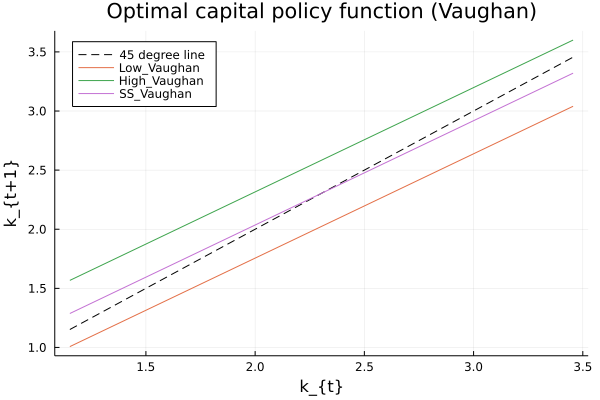
\includegraphics[scale=0.5]{kpol_Vaughan.png}
		\caption{Optimal policy function for capital from Vaughan method}
	\end{figure}
	
	\begin{figure}[htbp]
		\centering
		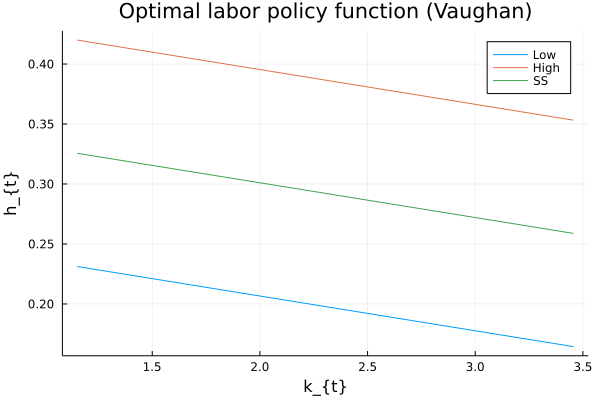
\includegraphics[scale=0.5]{hpol_Vaughan.png}
		\caption{Optimal policy function for labor from Vaughan method}
	\end{figure}
	
	
\end{document}